\documentclass[twocolumn, a4paper, 9pt]{UECIEresume}

\usepackage[dvipdfmx]{graphicx}
\usepackage{graphicx}
\usepackage{amsmath}
\usepackage{txfonts}
\usepackage{epsfig}
\usepackage{tabularx}
\usepackage{amssymb}
\usepackage{url}
\usepackage{mediabb}
\newcommand{\bhline}{\noalign{\hrule height 1pt}}
\newcommand{\ab}{\allowbreak}

\title{Twitterを用いた携帯端末における個人認証の多要素化に関する研究}
\date{平成 26 年 02 月 10 日}
\affiliation{総合情報学科 セキュリティ情報学 コース}
\supervisor{高田 哲司 准教授}
\studentid{1010086}
\author{高浪 悟}
%\headtitle{平成 yy 年度 総合情報学科 卒業論文中間発表}
\headtitle{平成 25 年度 総合情報学科 卒業論文発表}
%\headtitle{平成 yy 年度 総合情報学科 修士論文中間発表}
%\headtitle{平成 yy 年度 総合情報学科 修士論文発表}

\begin{document}
\maketitle

\section{はじめに}\label{introduction}
高性能な携帯端末の普及\cite{idcsmartphone}により,個人や決済にかかわる重要な情報を持ち歩くことが一般化しつつあり,警視庁もスマートフォンの電話帳データや位置情報などを不正に送信するアプリケーションソフトウェア(以下,アプリと略す)への注意喚起を行っている\cite{keishichoSmartphone}.

Apple社が自社の製品であるiPhone 5Sに指紋認証機能を搭載したり,通常のスクリーンロックの多要素認証化を行うHidden Lock\cite{hiddenLock}やアプリの起動などに対しても個別にロックを設定可能なAppLock\cite{applock}等のアプリが配布されるなど,より多くの場面で個人認証の強化をはかる動きがある.

携帯端末におけるロック解除や,金融やWebサービスの多要素認証では,例えばハードウェアトークンを用いた所有物認証など,知識認証以外の手法を導入する例が多くみられるが,本研究では,ユーザからみた手軽さやサービスプロバイダが負担するコストなどの面から,知識認証を複数種類組み合わせる認証の多要素化手法を提案する.
多要素認証を導入すれば当然ながらユーザの負担は増えるが,その負担増を最低限にするため,新たな操作法を習得する必要がなく,秘密情報の生成/記憶負担にも配慮した認証手法を考案する.

\section{関連手法}
携帯端末における個人認証を強化する手法としては,Googleの開発している携帯端末向けプラットフォームであるAndroidでは第\ref{introduction}章で述べたAppLock\cite{applock}や生体認証を利用できるPassBoard\cite{passboard}などが存在する.

ライフログやSNSを認証に用いる手法に関して,西垣ら\cite{西垣正勝:2006-03-15}は,ユーザの生活履歴を用いて認証を行う手法を提案し,そのプロトタイプとしてEメールを用いたシステムの構築と実験を行った.Eメールによる認証は,「最近のメールかどうか」をユーザに回答させるというプロセスで行われた.その際,人間の記憶の曖昧性を取り除くための手法として,最近と過去どちらともいえないような期間のメールを利用しない,例えば「8日前から29日前までのメールは質問の中に出てきません」と明示することでユーザが直感的に回答を行えるようにした.
また,Nemotoら\cite{nemoto:2006-03-15}は,Twitterのダイレクトメッセージ\footnote{特定のユーザ宛に,一対一で送信された文章のこと.閲覧可能な人物は,自分と相手のみである.}(DM)機能を用いて,定期的に質問を投げかけることでその回答を秘密情報とし,認証を行うシステムを提案した.
質問の内容は「2月15日の昼食は?」といった文面で構築され,Twitterのダイレクトメッセージ機能により送信され,回答も同機能を用いて行う.

\section{提案システム}
第\ref{introduction}章での議論を基に,携帯端末の個人認証強化を目的とした,以下の特徴を持つ個人認証手法を実装した.
\begin{itemize}
  \item 携帯端末の画面ロックにおける個人認証を想定する.既存のシステムはPINによる1要素認証だが,これに提案する認証を追加して2要素認証とする
  \item 秘密情報は,利用者が既知であるライフログやSNSの情報としてTwitterのツイートを利用する
  \item 認証操作は回答選択方式で,既知の操作方法と同一にする
\end{itemize}

\subsection{認証操作}
本システムでは認証のために新たな操作を覚える負担を考慮し,認証操作に既存の携帯端末向けOSで既に実装されているロック画面中の通知機能を利用する際の操作と同等の操作で認証操作が可能なユーザインターフェイス(UI)をiOSアプリとして実装した.

通知の表示画面を模した認証画面(図\ref{notifauthTest}左)では,10個のツイートの本文と,当てはまるものがなかった場合に選択する「No match」の11つの候補を表示している.
その中から,ユーザが正解だと判断した回答を選択するとPIN入力画面に遷移する.

PIN入力画面(図\ref{notifauthTest}右)は既存のUIと同一であり,入力確定後に認証結果が表示される.両者の回答が共に正解であれば、認証に成功する仕組みとなっている.

\subsection{秘密情報の設定}
本提案では2種類3方法の秘密情報を検討し,実装した.
1つは既存の認証と同様の固定秘密であり,もう1つは規則を秘密情報とする可変秘密である.
可変秘密の方法を採用した理由は,定期的な秘密情報の変更を能動的に行う必要が低減されるからである.

それぞれの秘密情報の設定方法は以下の通りである.

\subsubsection{Auto Mode Type Term}
可変秘密の1つであり,特定の期間を秘密とする手法である.
つまり秘密である特定期間につぶやかれたツイートが秘密情報となる.
期間の指定方法は開始する時期と期間(例: 1週間前から3日間)になる.
設定時もしくは前回の認証時から新しく投稿されたツイートも秘密情報の候補として含まれ,ツイートを選択した後は従来のPIN認証との比較のため4桁のPINを入力する.

\subsubsection{Auto Mode Type Cycle}
可変秘密のもう1つの提案であり,特定期間を秘密とする点では前述の手法と同じであるが,秘密情報の指定は曜日と時間(例: 水曜日の23時台)となる.
新しく投稿されたツイートの扱いと認証の手順はAuto Mode Type Termに準ずる.

\begin{figure}[ht]
  \begin{minipage}{0.49\hsize}
    \begin{center}
      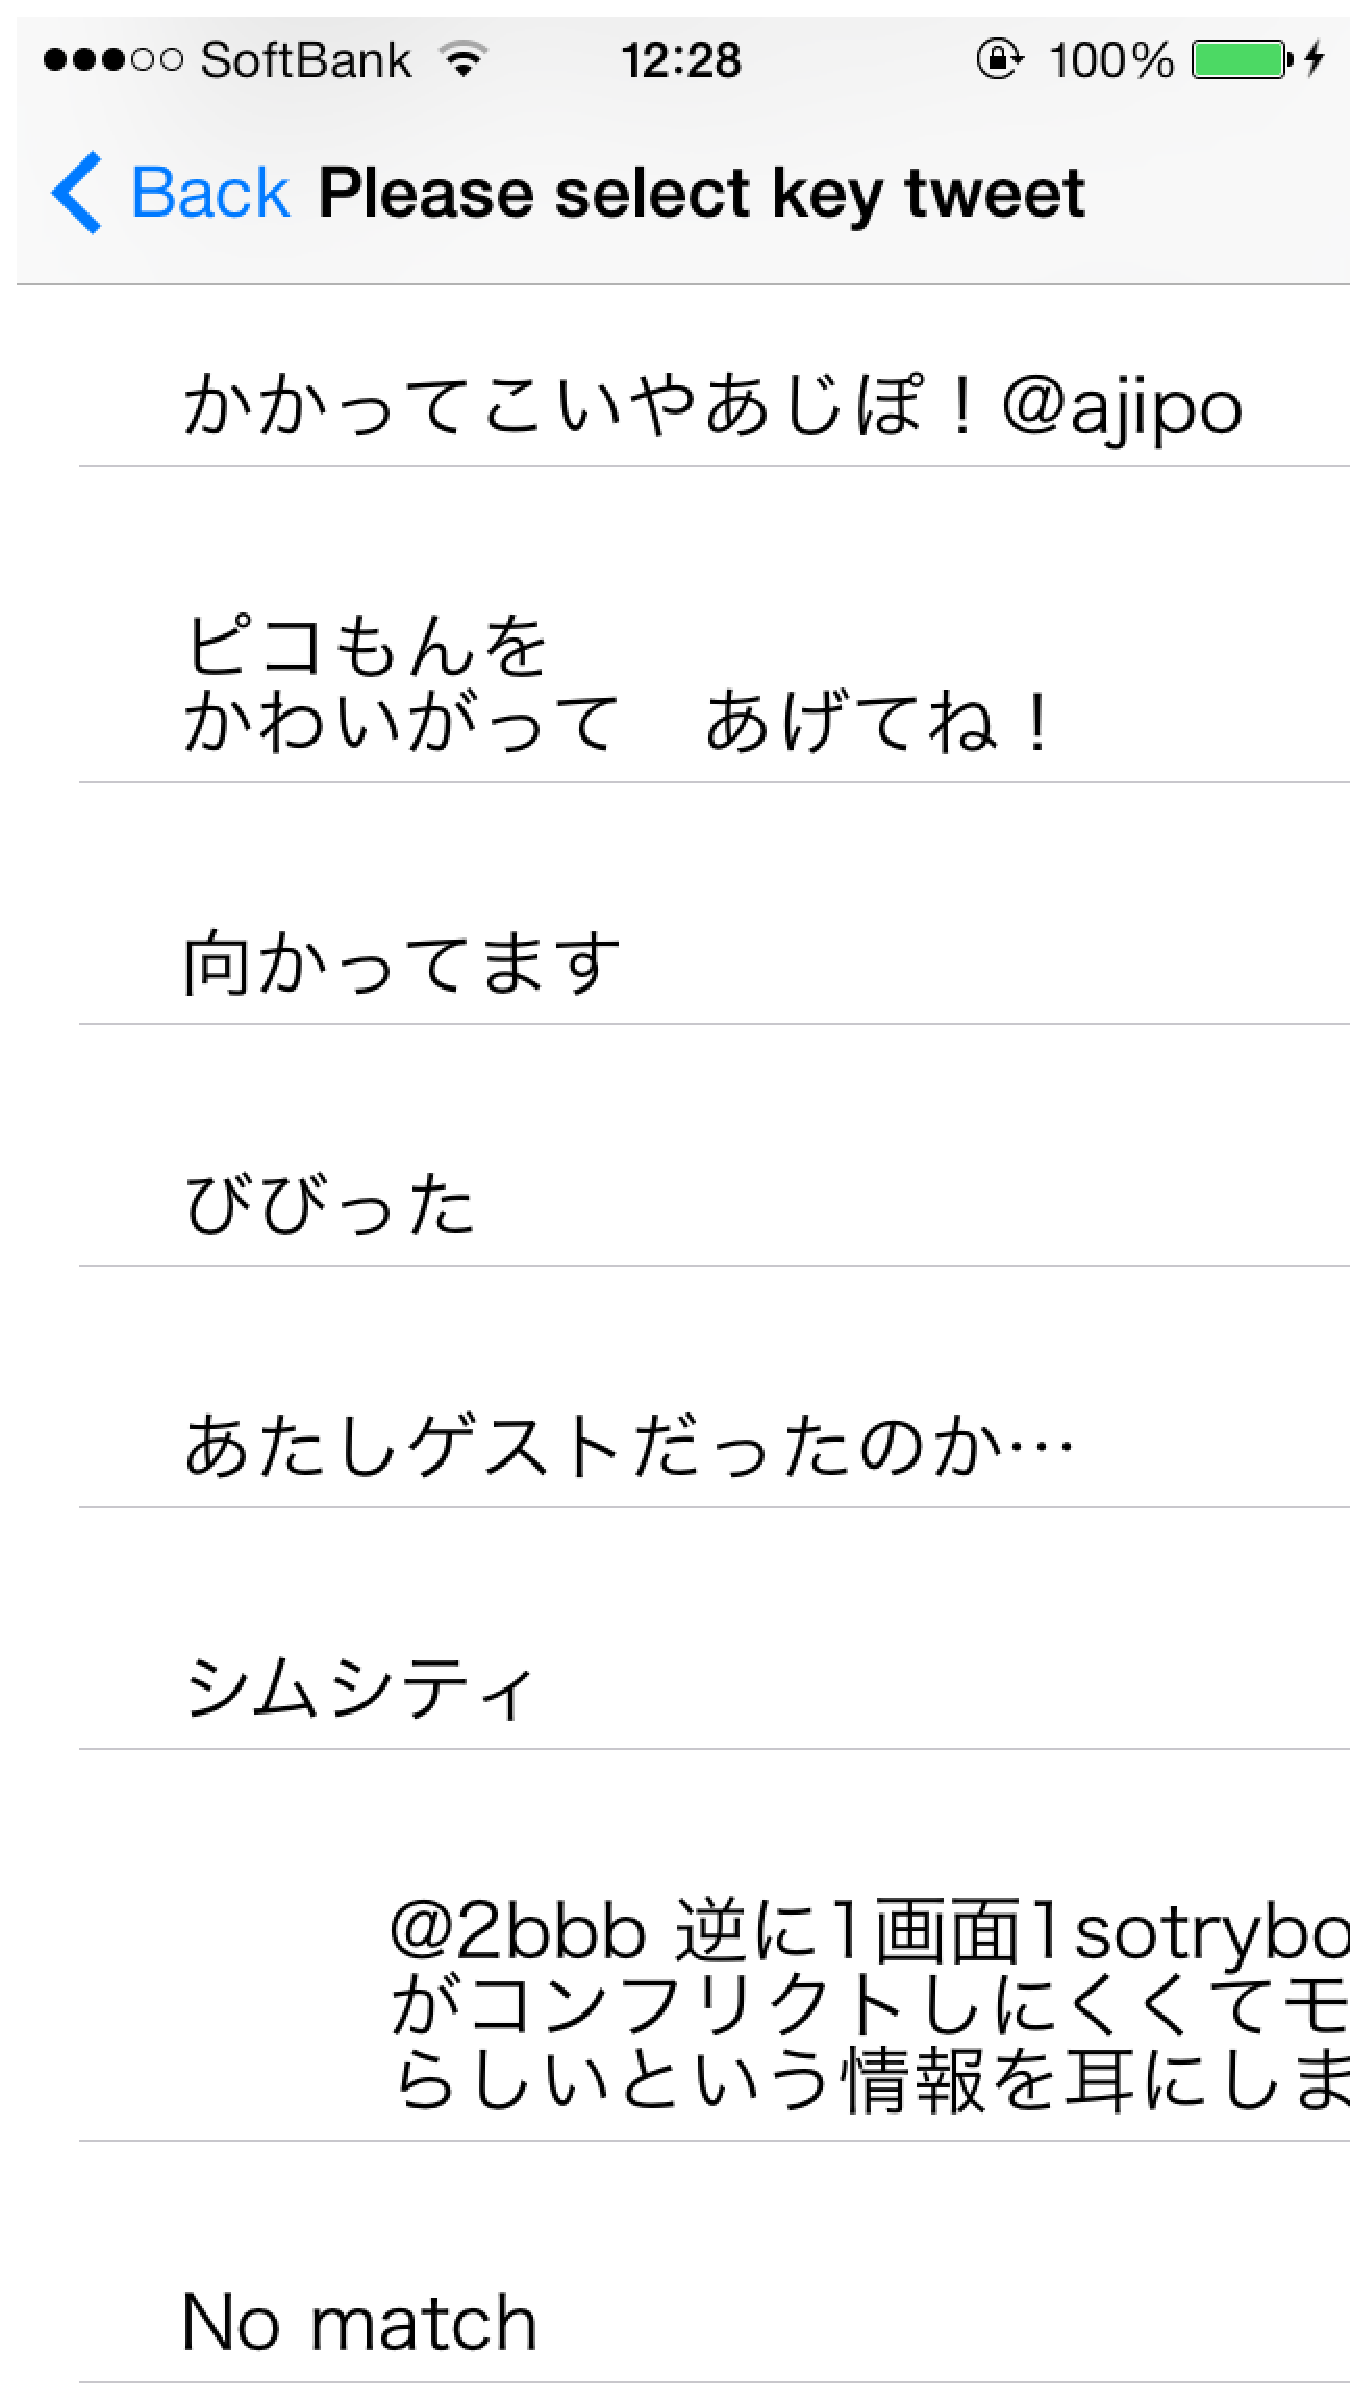
\includegraphics[width=40mm]{img/notifauthNotificationTest.eps}
    \end{center}
  \end{minipage}
  \begin{minipage}{0.49\hsize}
    \begin{center}
      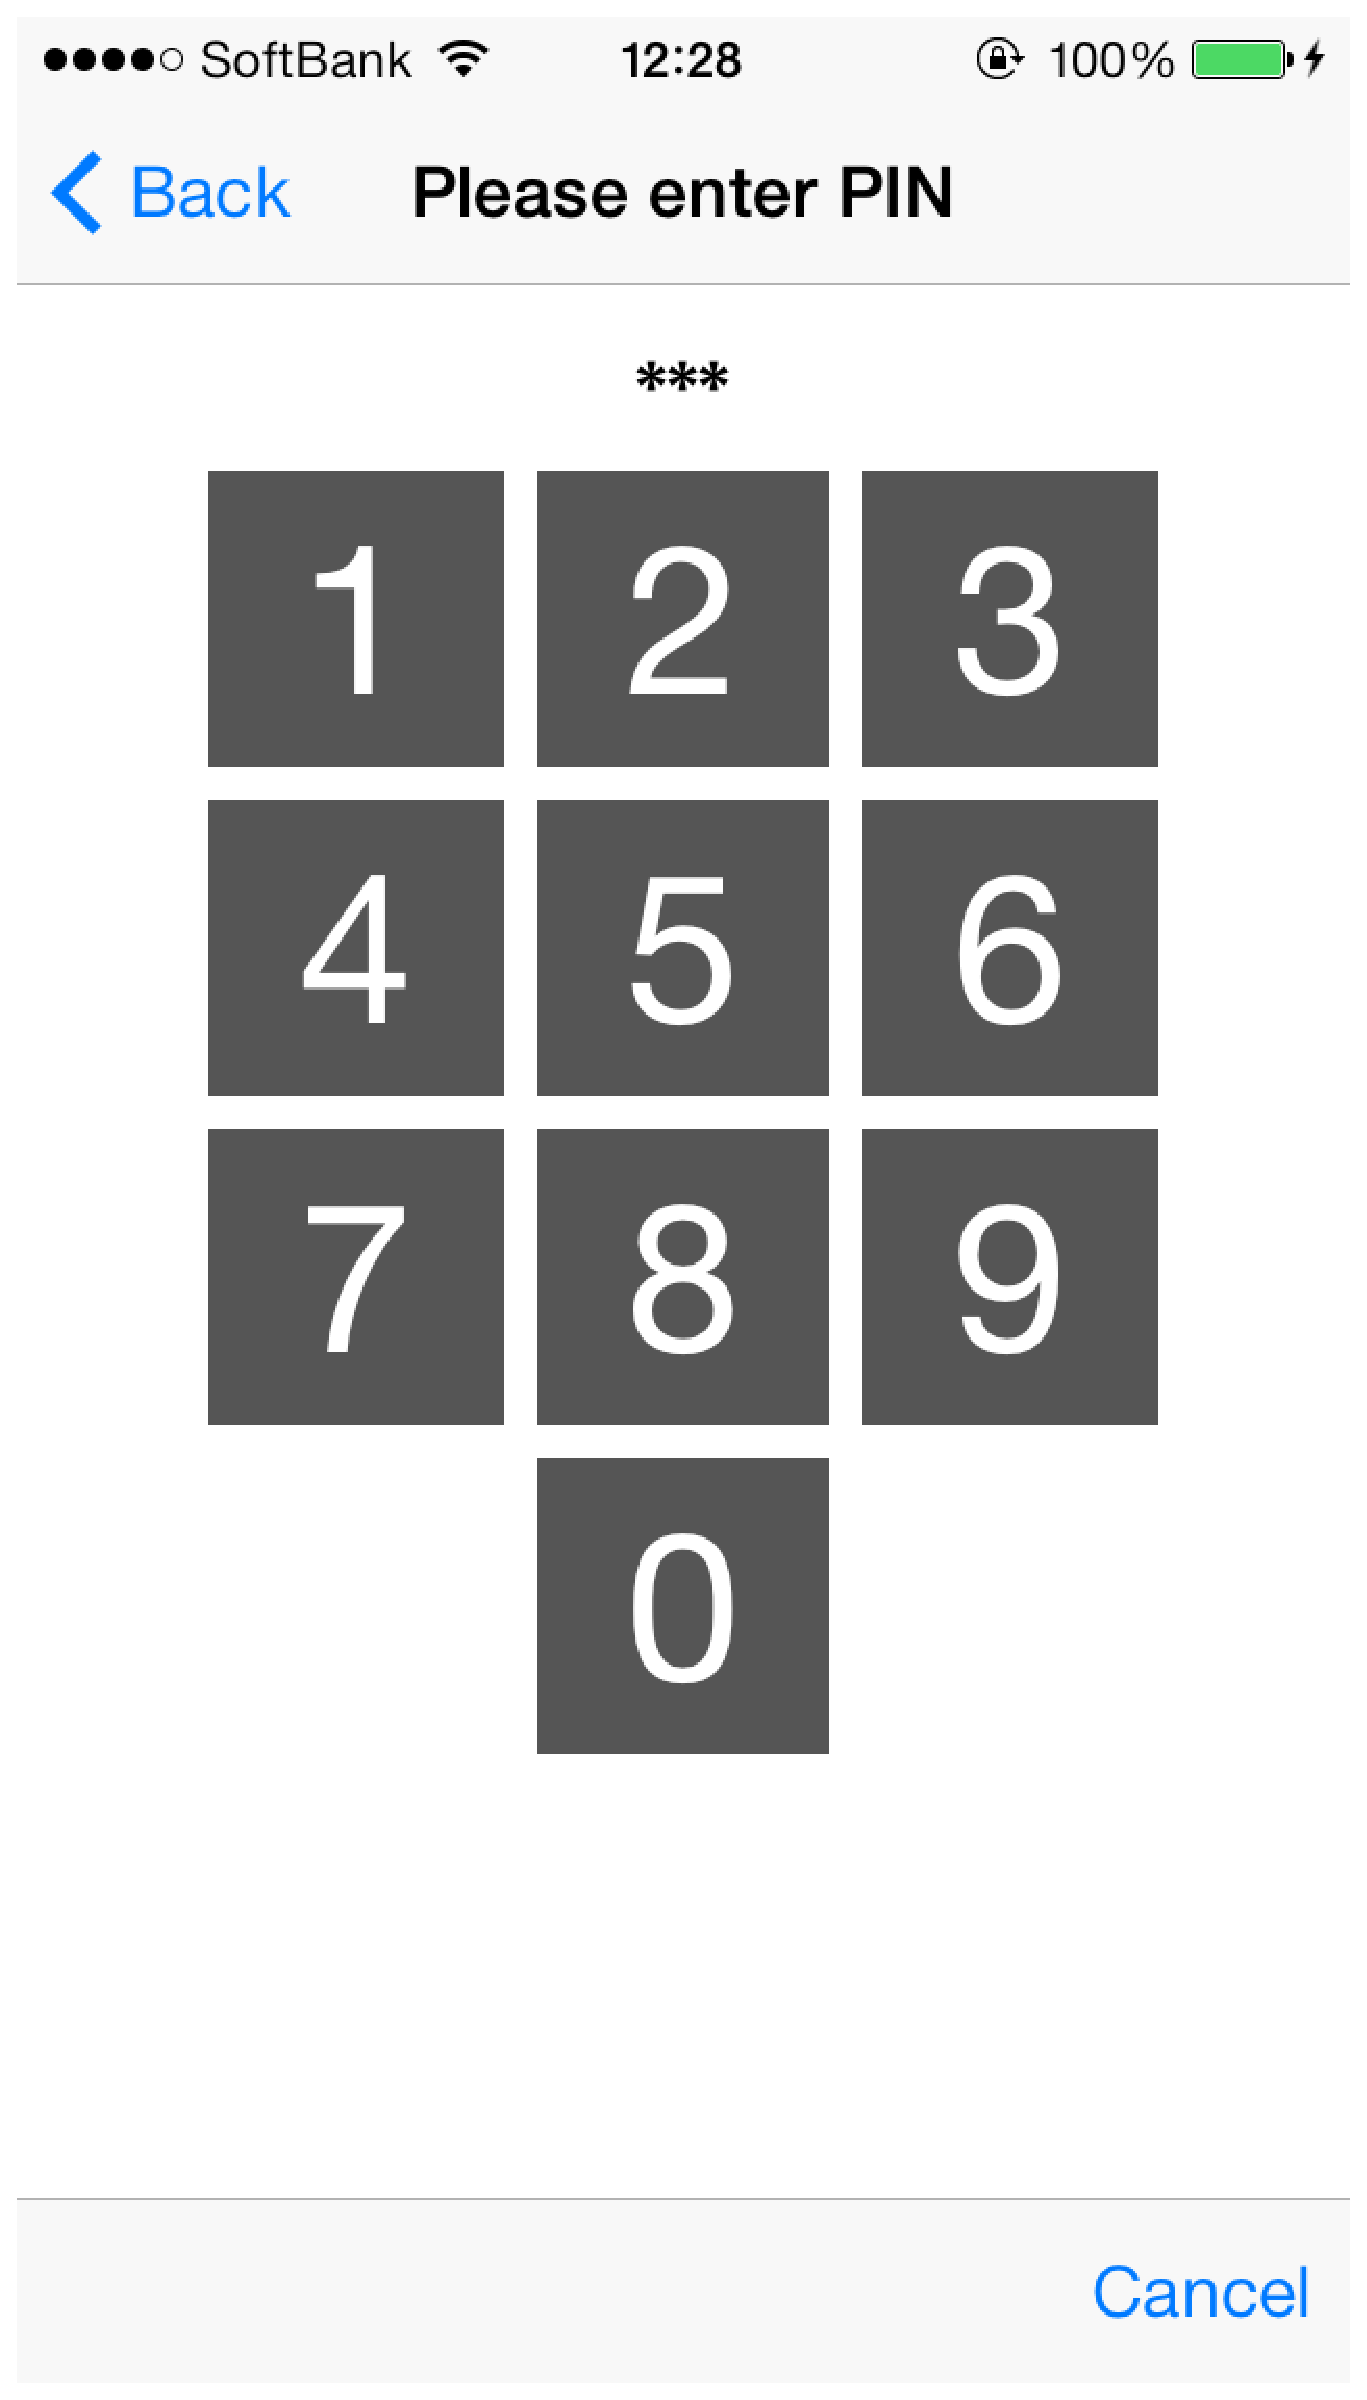
\includegraphics[width=40mm]{img/notifauthPINTest.eps}
    \end{center}
  \end{minipage}
  \caption{2種類の認証操作画面}
  \label{notifauthTest}
\end{figure}

\subsubsection{Manual Mode}
利用者は、最新ツイート200件の中から、任意の1ツイートを秘密情報として選択する.不正解となるツイートはそれ以外の199件からランダムに抽出される.

\section{利用可能性に関する被験者実験}\label{result}
提案手法の利用可能性について被験者により評価実験を行った.
実験は提案3手法の他に比較対象として5桁の暗証番号認証を加えた4種類で実施した.
各認証手法は8日間で4回の認証を実施させ,認証成否と認証時間を測定した.
被験者は15名で性別ならびに年齢構成は表\ref{testee}の通りである.
また,4種の評価実験のうち2種の実験を終了した時点で中間アンケートを,全て終了した後に最終アンケートを実施した.
実験結果は表\ref{eachResult}に示す.

\begin{table}[ht]
  \caption{被験者の属性分布}
  \label{testee}
  \begin{center}
    \small
    \begin{tabular}{rrr}
      \bhline
       & 男性 & 女性 \\ \hline
      20代 & 10人 & 1人 \\
      30代 & 1人 & 2人 \\
      40代 & 1人 & - \\
      \bhline
    \end{tabular}
  \end{center}
\end{table}

\begin{table}[ht]
  \caption{各手法における認証成功率と認証時間}
  \label{eachResult}
  \begin{center}
    \small
    \begin{tabular}{rrr}
      \bhline
      手法名 & 認証成功率(\%) & 認証時間(秒) \\ \hline
      Auto Mode Type Term & 51.79 & 22.14 \\
      Auto Mode Type Cycle & 27.59 & 22.95 \\
      Manual Mode & 94.12 & 10.74 \\
      PIN Mode & 94.34 & 2.56 \\
      \bhline
    \end{tabular}
  \end{center}
\end{table}

\section{考察}\label{discussion}
Manual Modeの認証時間はPIN Modeの4倍程度かかっており,特に一日に何度も認証を行う可能性の高い携帯端末では,利便性の面において改善が必要だと考えられる.
しかしながら,アンケートによる比較では,使いやすさと憶えやすさ両方の項目で,Manual Modeが4パターン中最も優れているとした被験者が多かったことと,「認証にかかる時間はどのように感じましたか?」の問いに対する被験者の主観による評価はPINとManualで有意差がみられなかったことから,ユーザにとっては5桁の暗証番号と同程度の負荷,つまり安全性を強化するために「1種類の秘密情報で秘密空間を拡大する」のと,「2種類の秘密情報(PIN+ツイートによる11選択)を利用して安全性を強化」するのとで利用者が感じる負担は同程度だと言うことがわかった.

自動で設定する2手法(Auto Mode Type TermとAuto Mode Type Cycle)では,PIN認証と比べ大きく認証成功率が劣っているが,これはアンケートの内容から「設定情報は覚えているがそれに当てはまるツイートを選べない」という問題によるものであるといえる.この問題に対する改善策として,既存手法\cite{西垣正勝:2006-03-15}で対策されているのと同様に,独立した一つの情報,本システムの場合は1ツイートに対して2-4択で正解の選択肢を答えさせ,それを複数回繰り返すという方法が考えられる.
既存手法ではこれに加え,曖昧な記憶による認証の失敗を防ぐため,はっきりと覚えている情報のみを認証に用いた.
この2手法を導入することで,Auto Modeによる秘密設定における認証成功率の向上が可能になると考える.
自動で設定する2手法では,定期的な秘密情報の変更を能動的に行う必要が低減されることや,時間経過によるエントロピの増加などの利点が考えられたが,今後はそれらを活かすために認証成功率を上昇させることが最優先であると考えている.

\section{おわりに}\label{finish}
本研究では,現在の携帯端末の普及と情報の集約に伴う個人認証強化の必要性を議論し,知識認証の多重化による多要素認証を提案した.
その際,既存の知識と操作を用いてユーザの負担を減らすべく,ライフログやSNSの情報を認証に使うことの有用性などを検討し,Twitterの情報を用いた携帯端末向け個人認証の多要素化手法の提案とプロトタイプシステムの実装を行った.
また,実装したシステムを用いて被験者実験を行い,利用可能性について評価を実施した.

%{\small
\bibliographystyle{unsrt}
\bibliography{bibtex}
%}

\end{document}